\section{Introduction}
\label{sec:intro}

% QC offers speedups
% - Source of speedup: Oracle, run coherently

Quantum computers offer unique capabilities that can be used to
program substantially faster algorithms compared to those written for
classical computers. For example, Grover's search algorithm \cite{grover1996,grover1997}
can query unstructured data in sub-linear time (compared to linear
time on a classical computer), and Shor's algorithm \cite{shors} can factorize a
number in polynomial time (compared to the sub-exponential time for the
best known classical algorithm).

It is well known that quantum computers provide quantum supremacy.
Most quantum algorithms are not classically simulatable because of the property.
Unfortunately, the current quantum computers are limited and noisy, 
so it is hard to test the algorithms in a quantum computer as well as a classical computer.
However, an algorithm not being efficiently simulatable in a classical computer does not mean
that it is not efficiently provable in the computer.
An analogy is that for a lottery system, we can easily prove that someone can win a lottery in a certain probability,
but it is extremely hard to find out who will win the lottery.
For example, simulating Shor's algorithm \cite{ddsim} is hard, but its property has been proved
on paper and in Coq \cite{shorsprove}.
It is highly likely that we can discover an efficient and automatic proof framework
to extract and certify the properties for quantum algorithms.

Unfortunately, previous quantum proof frameworks \cite{qhoare, quantumseparation, VOQC, qbricks}
permit proofs with many human-interactions.
It is unlikely that algorithms can be proved automatically in these frameworks.
For example, the Shor's algorithm proof in Quantum Separation Logic \cite{quantumseparation}
was proved by assuming that the property of the oracle loop was given and the last part was omitted.
The complete Shor's algorithm proof in VOQC \cite{VOQC} 
was done by intelligent researchers who spent two years.
The reason is that these systems specify quantum programs with quantum states, 
such as density matrices and high denominational Hilbert spaces.
These structures cannot be effectively captured in a classical computer.
Although there is a mechanism \cite{10.1145/3453483.3454061}
to reduce the complexity of representing these quantum states,
the key is that they lack the establishment of "computer understandable" axioms and theories to permit
proof automation in verifying quantum algorithms.
More sadly, the establishment is itself a hard problem.

\begin{figure}[t]
  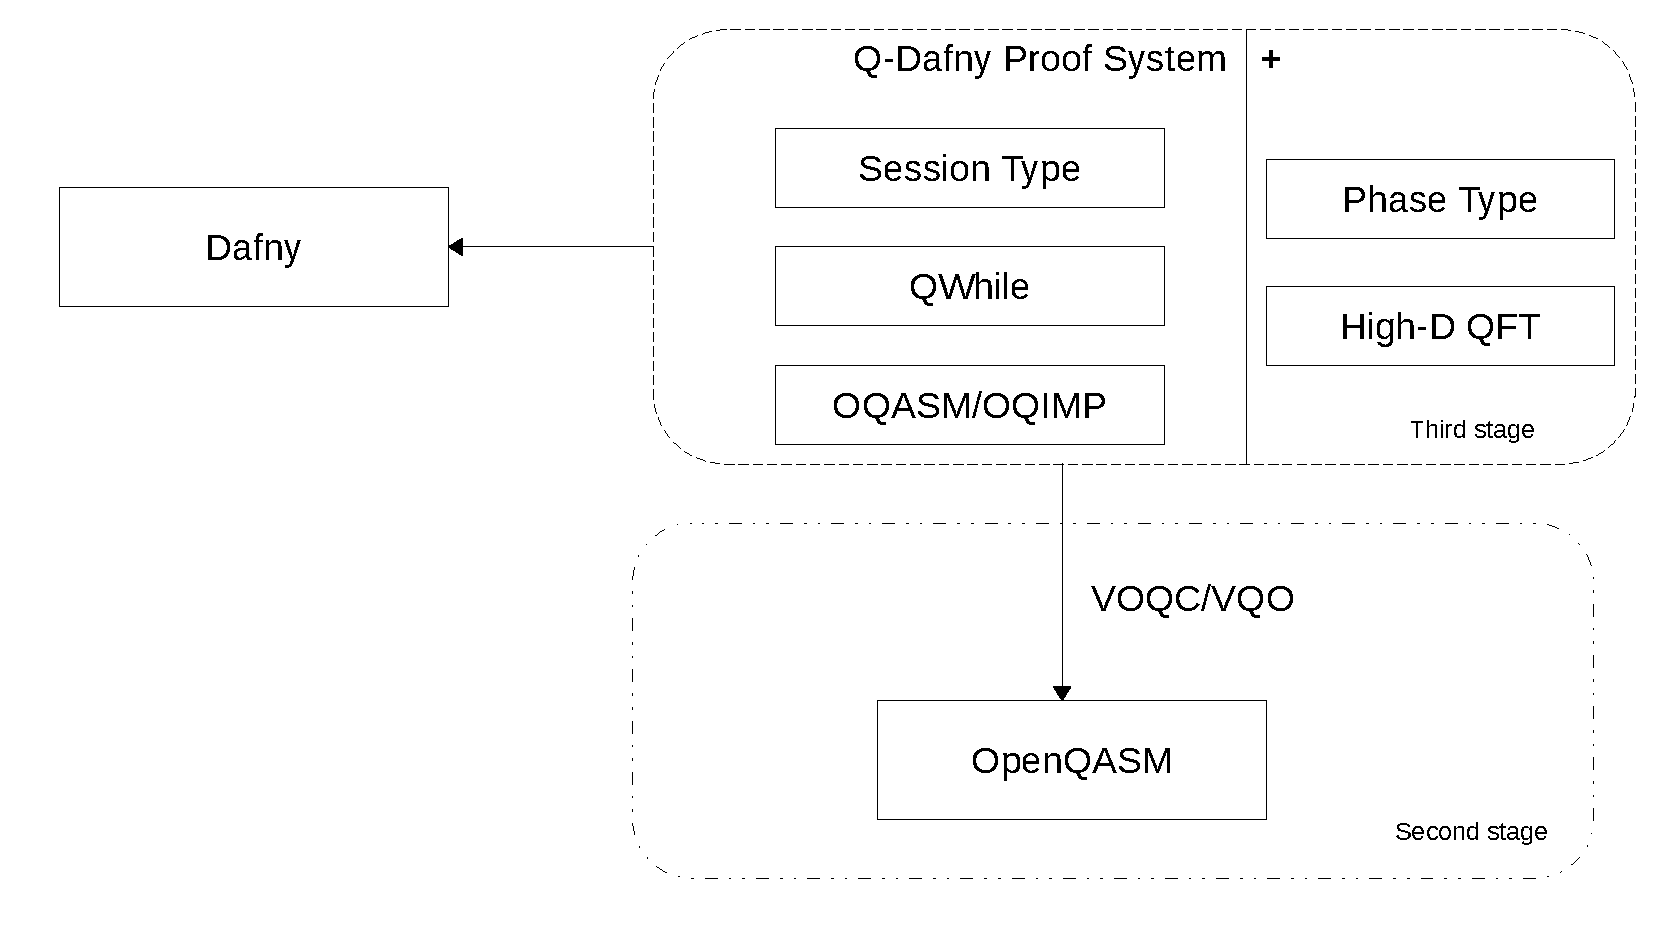
\includegraphics[width=.75\textwidth]{stage}
  \caption{QNP Development Stages and the Key Aspects}
\label{fig:arch}
\end{figure}

On the other hand, there are many classical data state structures that have already had good proof automation theorems,
such as first order array, linked list, and graph theories. 
If we can connect quantum states with these existing classical theories, 
many quantum algorithms can be reasoned by these existing classical proof theories. 
We propose Quantum Natural Proof (QNP), a system to map quantum algorithms 
to classical programs that run on the classical Hoare Logic style proof system, 
and efficiently and automatically certify quantum program properties.
The key observation is that although quantum algorithms running on quantum computers have quantum supremacy,
the structures of many algorithms are simple. 
In addition, the states appearing in these algorithms can be mapped to classical array structures.

\Cref{fig:arch} provides the QNP development plan. 
In the first stage, we develop the Q-Dafny proof system including a quantum language (QWhile) 
that contains operations for writing oracles (QQASM/OQIMP),
a type system to record the qubit state forms for easing property proofs, 
as well as a proof system built on top of the classical Hoare Logic array theory.
In addition, Q-Dafny is compiled to Dafny, 
such that a quantum program with its user-defined properties is compiled to Dafny with additional auto-generated Q-Dafny axioms.
The program properties are eventually automatically proved in Dafny with the auto-generated Q-Dafny axioms.
The second stage is to compile programs in QWhile, as a quantum language, to ones in OpenQASM,
such that a verified QWhile program can be run on a quantum computer. 
The third stage upgrades Q-Dafny's type system to track not only quantum state bases but also phases.
Then, a multi-denominational quantum Fourier transformation (High-D QFT) theory can be built on top of the upgraded type system,
so that the Q-Dafny+ proof system is capable of defining advanced quantum algorithms that rely on the High-D QFT theory.
One example is quantum signal processing \cite{Low_2017}.

In this document, we mainly focus on the explanation of the first stage. Here are three key aspects.

\myparagraph{Based on Hoare Logic Array Theory}
We first select the target mapping classical data structure -- arrays, because of two reasons.
First, quantum states can be represented by arrangement of quantum qubits which usually can be thought of as special arrays.
Thus, quantum entanglement of some qubits can be thought as some properties defined on the qubits, 
such that once a qubit is measured, the other qubits consequentially perform some state changes.
Second, classical array structures are the most commonly used data structure 
that has many proved theories and axioms, which does not rely on array sizes, for proof automation;
while other data structure automated proof theories (axioms), such as linked lists, 
finish a property proof by an exclusive proof search on the list of elements in the data structure \cite{DBLP:conf/pldi/Qiu0SM13}.
To represent $n$ qubits as an array in Q-Dafny and verify a property on them, sometimes,
we create a $2^n$ array to capture the entanglement relations among the qubits
and expect the array theory to prove the property symbolically regardless the array size.

\myparagraph{Using a Session Type System to Classify State Forms}
Consequentially, representing quantum states by arrays has its limitations.
Conceptually, state representations in the Q-Dafny proof system
implies the arrange of a set of axioms that facilitate program property proof automation.
Nevertheless, quantum states are high dimensional while arrays are linear.
This fact almost always indicates that the set of axioms might be huge 
and the way of applying the axioms for proof automation is not linear,
so that the proof automation faces major obstacles. 

To overcome these obstacles, we identify three different quantum state representations (\Cref{fig:vqir-state}) in Q-Dafny, 
which are associated with different axioms for proof automation.
Then, the Q-Dafny session type system tracks the transformation of different state 
representations for different \textit{sessions}, collections of qubit array segments that are possibly entangled.
Conceptually, the different state representations guarantee the Q-Dafny proof system can be expressed
in terms of the Hoare Logic array theory.
In compiling Q-Dafny to Dafny,
for proving a local property for a session, we generate and identify different axioms for different state representations,
and we also generate axioms that handle the transformation between state representations.

\begin{figure}[t]
{\small
  \begin{lstlisting}[language=C++,xleftmargin=4 mm]
method Shor ( a : int, N : int, n : int, x : Q[n], y : Q[n] )
 requires (n > 0)
 requires (1 < a < N)
 requires (N < 2^(n-1))
 requires (gcd(a, N) == 1)
 requires ( type(x) = Tensor n (Nor 0))
 requires ( type(y) = Tensor n (Nor 0))
 ensures (a^xv mod N == yv)
 ensures (gcd(q, t) == 1)
 ensures (is_even(t))
 ensures (a^(t/2) + 1 divides N || a^(t/2) - 1 divides N)
 //ensures (r.pos > (4 * e^(-2) / PI ^ 2) / (Nat.log2 N)^4)
{
  x *= H ;
  y *= cl(y+1); //cl might be omitted.
  for (int i = 0; i < n; x[i]; i ++)
    invariant (0 <= i <= n)
    invariant (saturation(x[0..i]))
    invariant (type(x[0..i],y) = Tensor n (ch (2^i) {k | j baseof x[0..i] && k = (j,a^j mod N)}))
    //psum(k=b,M,p(k),b(k)) = sum_{k=b}^M p(k)*b(k)
    invariant ((x[0..i],y) == psum(k=0,2^i,1,(k,a^k mod N))) 
  {
    y *= cl(a^(2^i) * y mod N);
  }

 M z := measure(y);//forall x in x[0..n), valid(x) ==> z.base = a^(x.base) mod N
 x *= RQFT;
 M r := measure(x); //r is r.pos and r.base
 int t := conFrac(r); //continued fraction of r.base and maintain r.pos (probability)
 
}
  \end{lstlisting}
}
\caption{Shor's Algorithm in Q-Dafny}
\label{fig:shorexample}
\end{figure}


\myparagraph{Enabling Complicated Oracle and Reflection Operations}
The first stage session type system tracks only qubit bases.
As a consequence, the set of quantum algorithms that are efficiently reasonable has the scheme $\texttt{QFT};U;\texttt{QFT}^{-1}$,
where $\texttt{QFT}$ and $\texttt{QFT}^{-1}$ are Hadamard or QFT gates that switch qubits array state forms between normal and superposition, $U$ is an arbitrary combination of QWhile operations that use Hadamard or QFT gates in a manageable manner.
For rich expressiveness, we permit two kinds of managed operations that might involve Hadamard or QFT gates: 
oracle assignments written in OQASM/OQIMP and quantum reflection operations (\texttt{amplify} and \texttt{diffuse} in \Cref{fig:vqimp}).
The concept of "management" refers to the fact that there is a type system in OQASM/OQIMP to ensure the use of Hadamard or QFT gates do not cause entanglement, as well as the Hadamard or QFT gate usage in quantum reflections has a fixed implementation, such that its semantics is well-known and its property reasoning is captured by Q-Dafny.

Almost all near term quantum algorithms are definable in terms of the above scheme, such as GHZ, Grover's, Shor's, and Childs' Boolean equation algorithms.
To prove properties about advanced quantum algorithms, the session type system needs to track qubit phases, which will complicate its design, and it is the major task of stage 3 in the QNP development.

















